\documentclass[10pt]{beamer}

% =========================
% Theme (sobre / académique)
% =========================
\usetheme{Madrid}
\usecolortheme{default}
\usefonttheme{professionalfonts}
\setbeamertemplate{navigation symbols}{}
\setbeamertemplate{footline}[frame number]

% =========================
% Packages
% =========================
\usepackage[utf8]{inputenc}
\usepackage[T1]{fontenc}
\usepackage{lmodern}
\usepackage{graphicx}
\usepackage{amsmath}
\usepackage{tikz}
\usetikzlibrary{shapes,positioning}
\usepackage[english]{babel}

% =========================
% Meta
% =========================
\title[AI-Guided Attack Surface Assessment]{Research Associate\\AI-Guided Attack Surface Assessment}
\author{Julien Soulé}
\institute{Interdisciplinary Centre for Security, Reliability and Trust (SnT)\\Services and Data Management (SEDAN)\\University of Luxembourg}
\date{\today}


% =========================
\begin{document}
% =========================

% -------------------------
\begin{frame}
    \titlepage
\end{frame}

% =====================================================
% AXIS 1 — UNDERSTANDING OF THE POSTDOC TOPIC
% =====================================================

\begin{frame}{Understanding the postdoc topic: context}
    \begin{itemize}
        \item Modern information systems expose a \textbf{large and evolving external attack surface}.
        \item This surface is composed of heterogeneous elements:
              \begin{itemize}
                  \item domains, IPs, certificates, services, cloud resources,
                  \item dependencies across organizations and providers.
              \end{itemize}
        \item In practice, attack surface assessment relies on:
              \begin{itemize}
                  \item multiple specialized tools,
                  \item iterative exploration driven by analyst expertise.
              \end{itemize}
        \item The project investigates how \textbf{AI techniques may assist and structure this process}.
    \end{itemize}

\end{frame}

\begin{frame}{Understanding the postdoc topic: objectives}

    \textbf{Reading of the project objectives}

    \vspace{0.2cm}
    \begin{itemize}
        \item Design an \textbf{AI-assisted orchestration layer} for attack surface assessment,
              centered on tools and analyst workflows rather than large datasets.
        \item Support analysts in:
              \begin{itemize}
                  \item selecting and sequencing assessment tools,
                  \item configuring scopes and parameters,
                  \item interpreting heterogeneous and mainly textual outputs.
              \end{itemize}
        \item Treat \textbf{simulation and emulation} as core research objects
              to study iterative exploration and decision-making.
        \item Aggregate observations into \textbf{structured and persistent representations}
              to maintain context across assessment steps.
        \item Provide \textbf{prioritized and explainable outputs}
              that support analyst reasoning and operational trust.
    \end{itemize}

    \vspace{0.3cm}
    \textbf{Positioning}

    \begin{itemize}
        \item AI as a \textbf{selective support to expert reasoning}, not an end-to-end replacement.
        \item Emphasis on robustness, traceability, and analyst-in-the-loop validation.
    \end{itemize}

\end{frame}


% =====================================================
% AXIS 2 — EXPECTED ROLE IN THE POSTDOC
% =====================================================

\begin{frame}{Expected role in the postdoc}
    \textbf{My understanding of the postdoctoral role}

    \vspace{0.2cm}
    \begin{itemize}
        \item Contribute to the \textbf{research design} of AI-based orchestration approaches.
        \item Develop and evaluate \textbf{prototypes} in interaction with real tools and data.
        \item Explore the combination of:
              \begin{itemize}
                  \item learning-based decision-making,
                  \item symbolic and structured representations,
                  \item practical constraints from cybersecurity operations.
              \end{itemize}
        \item Collaborate with researchers and practitioners to refine assumptions and metrics.
    \end{itemize}
\end{frame}

\begin{frame}{Understanding the postdoc topic: proposed workflow}

    \textbf{Illustrative workflow (derived from the project description)}

    \begin{columns}[T]
        \begin{column}{0.3\textwidth}
            \begin{center}
                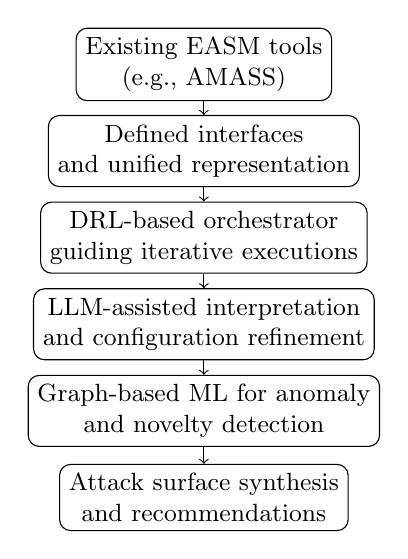
\begin{tikzpicture}[
                        node distance=1.1cm,
                        every node/.style={draw, rectangle, rounded corners, align=center, font=\small}
                    ]

                    \node (n1) {Existing EASM tools\\(e.g., AMASS)};
                    \node (n2) [below of=n1] {Defined interfaces\\and unified representation};
                    \node (n3) [below of=n2] {DRL-based orchestrator\\guiding iterative executions};
                    \node (n4) [below of=n3] {LLM-assisted interpretation\\and configuration refinement};
                    \node (n5) [below of=n4] {Graph-based ML for anomaly\\and novelty detection};
                    \node (n6) [below of=n5] {Attack surface synthesis\\and recommendations};

                    \draw[->] (n1) -- (n2);
                    \draw[->] (n2) -- (n3);
                    \draw[->] (n3) -- (n4);
                    \draw[->] (n4) -- (n5);
                    \draw[->] (n5) -- (n6);

                \end{tikzpicture}
            \end{center}
        \end{column}
        \begin{column}{0.65\textwidth}
            \vspace{1cm}
            \begin{itemize}
                \item The workflow emphasizes \textbf{orchestration and coordination},
                      not the replacement of existing tools or analysts.
                \item AI components are introduced incrementally to:
                      \begin{itemize}
                          \item structure observations,
                          \item guide exploration and tool usage,
                          \item support analyst decision-making.
                      \end{itemize}
                \item Human expertise remains central for validation,
                      interpretation, and trust.
            \end{itemize}
        \end{column}
    \end{columns}

\end{frame}


% =====================================================
% AXIS 3 — REMINDER OF RELEVANT PHD WORK
% =====================================================

\begin{frame}{Reminder of my PhD work (cyberdefense)}
    \textbf{PhD topic: organizational multi-agent systems for cyberdefense}

    \vspace{0.2cm}
    \begin{itemize}
        \item Modeling cyberdefense as a \textbf{sequential decision-making problem under uncertainty}.
        \item Design of multi-agent systems combining:
              \begin{itemize}
                  \item explicit organizational/symbolic models,
                  \item reinforcement learning (RL / MARL),
                  \item simulation and digital twins.
              \end{itemize}
        \item Focus on:
              \begin{itemize}
                  \item partial observability,
                  \item evolving environments,
                  \item analysis and interpretation of learned behaviors.
              \end{itemize}
    \end{itemize}
\end{frame}

% =====================================================
% AXIS 4 — PUTTING THIS BACKGROUND AT THE SERVICE OF THE POSTDOC
% =====================================================

\begin{frame}{Putting this background at the service of the postdoc}
    \textbf{Working hypothesis (open and discussable)}

    \vspace{0.2cm}
    \begin{itemize}
        \item Attack surface assessment can be viewed as:
              \begin{itemize}
                  \item an iterative exploration process,
                  \item driven by partial observations and expert hypotheses.
              \end{itemize}
        \item Some methodological ideas from my PhD may be relevant:
              \begin{itemize}
                  \item framing orchestration as a sequential decision problem,
                  \item using structured representations to maintain context,
                  \item analyzing agent behavior to support explainability.
              \end{itemize}
        \item These ideas would need to be adapted to:
              \begin{itemize}
                  \item EASM tools and data,
                  \item operational constraints,
                  \item analyst workflows.
              \end{itemize}
    \end{itemize}
\end{frame}

% =====================================================
% UPDATE — ROLE OF AI IN THE PIPELINE
% =====================================================

\begin{frame}{Where AI fits in the attack surface assessment pipeline}
    \textbf{AI as an enabling layer, not an end-to-end solution}

    \begin{columns}[T]

        \begin{column}{0.3\textwidth}

            \vspace{0.3cm}
            \begin{center}
                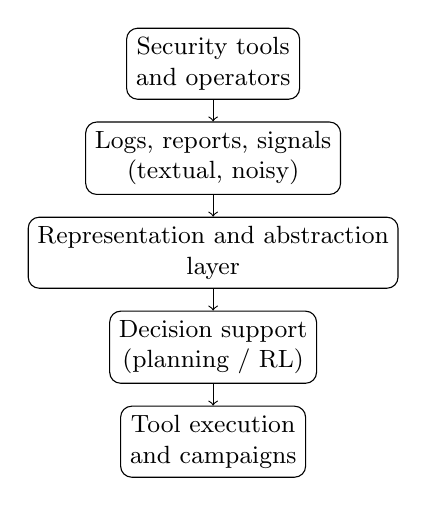
\begin{tikzpicture}[node distance=1.2cm, every node/.style={draw, rectangle, rounded corners, align=center, font=\small}]
                    \node (t1) {Security tools\\and operators};
                    \node (t2) [below of=t1] {Logs, reports, signals\\(textual, noisy)};
                    \node (t3) [below of=t2] {Representation and abstraction\\layer};
                    \node (t4) [below of=t3] {Decision support\\(planning / RL)};
                    \node (t5) [below of=t4] {Tool execution\\and campaigns};

                    \draw[->] (t1) -- (t2);
                    \draw[->] (t2) -- (t3);
                    \draw[->] (t3) -- (t4);
                    \draw[->] (t4) -- (t5);
                \end{tikzpicture}
            \end{center}

        \end{column}

        \begin{column}{0.6\textwidth}
            \vspace{0.2cm}
            \begin{itemize}
                \item AI does not replace existing tools nor expert analysts.
                \item Its role is to:
                      \begin{itemize}
                          \item structure heterogeneous outputs,
                          \item assist decision-making and prioritization,
                          \item support iterative orchestration of tools.
                      \end{itemize}
            \end{itemize}
        \end{column}

    \end{columns}

\end{frame}

% =====================================================
% UPDATE — TEXTUAL DATA AND LEARNING CHALLENGES
% =====================================================

\begin{frame}{Textual observations and learning challenges}
    \textbf{Identified difficulty}

    \vspace{0.2cm}
    \begin{itemize}
        \item Observations are often:
              \begin{itemize}
                  \item textual (logs, tool outputs, reports),
                  \item high-dimensional and noisy,
                  \item not directly suitable as RL states.
              \end{itemize}
    \end{itemize}

    \vspace{0.3cm}
    \textbf{Possible abstraction strategies (to be explored)}

    \begin{itemize}
        \item Extraction of \textbf{task-relevant signals} and summaries.
        \item Learned representations:
              \begin{itemize}
                  \item embeddings,
                  \item autoencoders,
                  \item constrained LLM-based encoders.
              \end{itemize}
        \item Hybrid approaches combining:
              \begin{itemize}
                  \item symbolic structures,
                  \item learned representations.
              \end{itemize}
    \end{itemize}
\end{frame}


% =====================================================
% UPDATE — RISKS AND MITIGATION
% =====================================================

\begin{frame}{Scientific and technical risks}
    \textbf{Identified risks and mitigation strategies}

    \vspace{0.2cm}
    \begin{itemize}
        \item \textbf{RL / MARL instability}
              \begin{itemize}
                  \item Mitigation: start with single-agent or hierarchical setups,
                        curriculum learning, strong baselines.
              \end{itemize}
        \item \textbf{LLM non-determinism and trust}
              \begin{itemize}
                  \item Mitigation: constrained prompting, fine-tuning,
                        symbolic post-processing.
              \end{itemize}
        \item \textbf{Simulation realism gap}
              \begin{itemize}
                  \item Mitigation: progressive validation against real tool behaviors
                        and expert feedback.
              \end{itemize}
    \end{itemize}
\end{frame}



% =====================================================
% AXIS 5 — INDICATIVE POSTDOC PLAN
% =====================================================

\begin{frame}{Indicative postdoc plan (open proposal)}
    % \textbf{Iterative and exploratory approach}

    % \vspace{0.2cm}
    % \begin{center}
    %     \begin{tikzpicture}[node distance=1.2cm, every node/.style={draw, ellipse, align=center}]
    %         \node (p1) {Problem\\formalization};
    %         \node (p2) [right of=p1, xshift=4.2cm] {Tool integration\\\& data structuring};
    %         \node (p3) [below of=p2, yshift=-1.1cm] {Learning-based\\orchestration};
    %         \node (p4) [left of=p3, xshift=-4.2cm] {Analysis \&\\feedback};

    %         \draw[->] (p1) -- (p2);
    %         \draw[->] (p2) -- (p3);
    %         \draw[->] (p3) -- (p4);
    %         \draw[->] (p4) -- (p1);
    %     \end{tikzpicture}
    % \end{center}

    % \vspace{0.2cm}
    \textbf{Progressive and risk-aware approach}

    \vspace{0.2cm}
    \begin{enumerate}
        \item \textbf{Tool analysis and workflow formalization}
              \begin{itemize}
                  \item study of existing EASM tools and expert practices,
                  \item identification of key decision points.
              \end{itemize}
        \item \textbf{Simulation and representation design}
              \begin{itemize}
                  \item emulation of attack surface scenarios,
                  \item abstraction of textual and heterogeneous outputs.
              \end{itemize}
        \item \textbf{Decision support and orchestration}
              \begin{itemize}
                  \item learning-based or rule-based guidance,
                  \item incremental integration of RL where appropriate.
              \end{itemize}
        \item \textbf{Evaluation, explainability, and feedback}
              \begin{itemize}
                  \item interaction with analysts,
                  \item refinement based on operational relevance.
              \end{itemize}
    \end{enumerate}

\end{frame}

% =====================================================
% AXIS 6 — EXPECTED DELIVERABLES
% =====================================================

\begin{frame}{Expected deliverables (indicative)}
    \textbf{Scientific deliverables}

    \begin{itemize}
        \item Publications on:
              \begin{itemize}
                  \item AI-assisted orchestration for attack surface assessment,
                  \item learning under partial observability in cybersecurity contexts,
                  \item structured representations and explainability for cyber analysis.
              \end{itemize}
        \item Target venues (depending on contributions):
              \begin{itemize}
                  \item AI / ML: AAMAS, IJCAI, AAAI, ICML (workshops or main tracks),
                  \item Cybersecurity: academic or applied security venues.
              \end{itemize}
    \end{itemize}

    \vspace{0.3cm}
    \textbf{Technical deliverables}

    \begin{itemize}
        \item Research prototypes (tool orchestration, analysis components).
        \item Reproducible experimental pipelines.
        \item Documentation supporting reuse and evaluation.
    \end{itemize}
\end{frame}

% =====================================================
% CONCLUSION
% =====================================================

\begin{frame}{Conclusion}
    \begin{itemize}
        \item A reading of the postdoc centered on AI-assisted, analyst-in-the-loop attack surface assessment.
        \item A proposed contribution grounded in prior work on decision-making under uncertainty in cyberdefense.
        \item An open and iterative plan, intended to be refined jointly with the SEDAN/SnT team.
    \end{itemize}

    \bigskip
    \bigskip
    \bigskip
    \centering
    \textbf{Thank you!}
\end{frame}

% =========================
\end{document}
